\begin{center}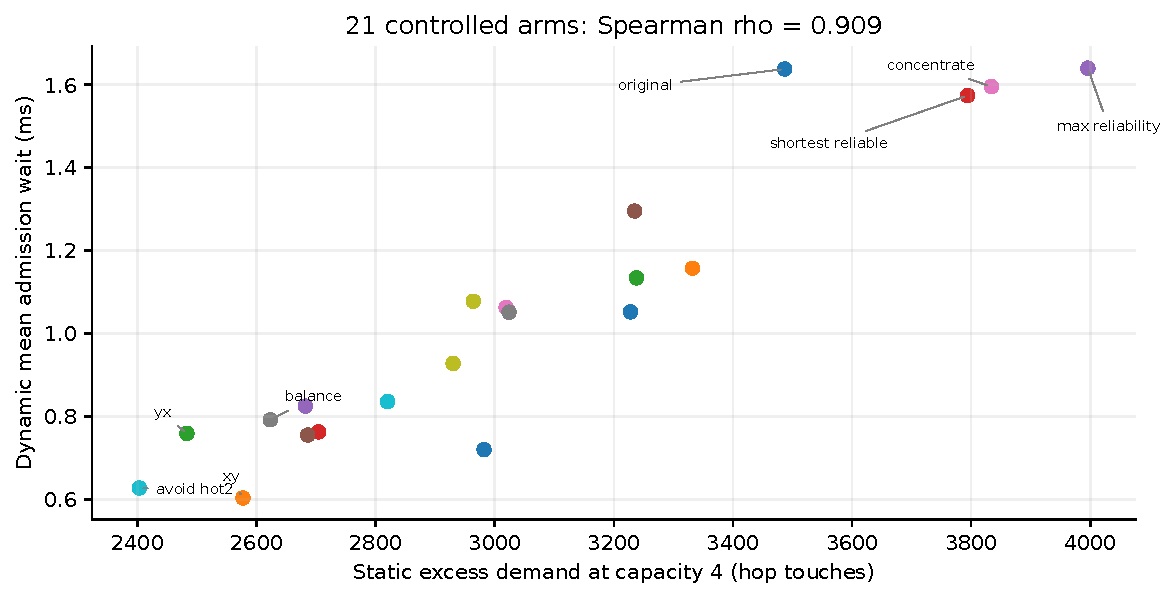
\includegraphics[width=\linewidth,height=0.37\textheight,keepaspectratio]{figures/mechanism.pdf}\captionof{figure}{Static layer demand predicts simulated waiting. Arms are controlled route alternatives sharing endpoints, not 21 independent workload samples.}\end{center}

\begin{center}\small
\begin{longtable}{lrrrr}
\caption{All 21 route alternatives, 30 seeds per policy. Values here are seed means; all SD values are in the unified data CSV.}\\
\toprule
Arm & Excess & ODG ms & Dynamic ms & Wait ms \\
\midrule\endfirsthead
\toprule
Arm & Excess & ODG ms & Dynamic ms & Wait ms \\
\midrule\endhead
original & 3487 & 1.5256 & 2.5701 & 1.6377 \\
xy & 2577 & 1.3401 & 1.4840 & 0.6034 \\
yx & 2483 & 1.3395 & 1.6275 & 0.7589 \\
shortest\_reliable & 3794 & 1.5377 & 2.5181 & 1.5736 \\
max\_reliability & 3996 & 1.5639 & 2.5966 & 1.6398 \\
mix\_p25\_s1 & 3235 & 1.4463 & 2.2112 & 1.2952 \\
mix\_p50\_s1 & 3019 & 1.3953 & 1.9666 & 1.0625 \\
mix\_p50\_s2 & 3024 & 1.3997 & 1.9519 & 1.0513 \\
mix\_p50\_s3 & 2964 & 1.4006 & 1.9826 & 1.0776 \\
mix\_p75\_s1 & 2820 & 1.3669 & 1.7241 & 0.8357 \\
rand\_shortest\_s1 & 3228 & 1.4062 & 1.9764 & 1.0521 \\
rand\_shortest\_s2 & 3332 & 1.4195 & 2.0885 & 1.1573 \\
rand\_shortest\_s3 & 3238 & 1.4194 & 2.0569 & 1.1340 \\
o1turn\_s1 & 2704 & 1.3547 & 1.6494 & 0.7624 \\
o1turn\_s2 & 2682 & 1.3497 & 1.7125 & 0.8248 \\
o1turn\_s3 & 2686 & 1.3489 & 1.6541 & 0.7550 \\
concentrate & 3834 & 1.5849 & 2.5589 & 1.5952 \\
balance & 2623 & 1.3336 & 1.6734 & 0.7918 \\
avoid\_hot1 & 2930 & 1.3999 & 1.8226 & 0.9277 \\
avoid\_hot2 & 2403 & 1.3431 & 1.5030 & 0.6273 \\
avoid\_hot3 & 2982 & 1.3642 & 1.6138 & 0.7196 \\
\bottomrule\end{longtable}\end{center}
{\footnotesize \href{https://github.com/sanjeevkrishnaa/Compiler-Driven-ACE/blob/codex/ace-scheduler-correctness/docs/latex/oct25_pre_golden/data/routing_mechanism.csv}{Complete CSV: routing\_mechanism}. }
